% \documentclass[11pt]{article}
% \usepackage[utf8]{inputenc}	% Para caracteres en español
% \usepackage{amsmath,amsthm,amsfonts,amssymb,amscd}
% \usepackage{multirow,booktabs}
% \usepackage[table]{xcolor}
% \usepackage{fullpage}
% \usepackage{lastpage}
% \usepackage{enumitem}
% \usepackage{fancyhdr}
% \usepackage{mathrsfs}
% \usepackage{wrapfig}
% \usepackage{setspace}
% \usepackage{calc}
% \usepackage{multicol}
% \usepackage{cancel}
% \usepackage[retainorgcmds]{IEEEtrantools}
% \usepackage[margin=3cm]{geometry}
% \usepackage{amsmath}
% \newlength{\tabcont}
% \setlength{\parindent}{0.0in}
% \setlength{\parskip}{0.05in}
% \usepackage{empheq}
% \usepackage{framed}
% \usepackage[most]{tcolorbox}
% \usepackage{xcolor}
% \colorlet{shadecolor}{orange!15}
% \geometry{margin=1in, headsep=0.25in}

\documentclass[11pt]{article}
 
\usepackage[margin=1in]{geometry} 
\usepackage{amsmath,amsthm,amssymb,scrextend}
\usepackage{fancyhdr}
\usepackage{graphicx}
\setlength{\headheight}{14pt}
\usepackage{xcolor}
\usepackage{color,soul}
\usepackage{gensymb}
\pagestyle{fancy}


\begin{document}
 
% --------------------------------------------------------------
%                         Start here
% --------------------------------------------------------------

\lhead{EE267 Virtual Reality}
\chead{Homework 3 Answers}
\rhead{Bohan Li}

\section{Theoretical Part}
\subsection*{(i) Vergence}
\subsubsection*{(a)}
The angle $\theta_{1,2}$ can be calculated using cosine rule:
\begin{align}
    \cos(\theta_1) &= \frac{|e_1 p_1|^2 + |e_2 p_1|^2 - |e_1 e_2|^2}{2 |e_1 p_1| |e_2 p_1|}\\[3pt]
    \cos(\theta_2) &= \frac{|e_1 p_2|^2 + |e_2 p_2|^2 - |e_1 e_2|^2}{2 |e_1 p_2| |e_2 p_2|}
\end{align}
The coordinates of the $e$ points are given as: \[e_1 = (-32,\ 0),\ e_2=(32,\ 0), \] therefore the distance are given as: \[|e_1 p_1| = 551,\ |e_2 p_1|=527,\ |e_1 p_2|=301,\ |e_2 p_2|=341,\ |e_1 e_2|=64,\] 
Thus the angles: \[\theta_1=6.32\degree,\ \theta_2=8.96\degree.\]

\subsubsection*{(b)}
For this part, we would need to rederive the expressions for the angles. Here we use the difference and inverse tan() functions. The angles are given:
\begin{align}
    \theta_1 &= \tan^{-1}(\frac{x_1+\text{ipd}/2}{z_1}) - \tan^{-1}(\frac{x_1-\text{ipd}/2}{z_1})\\
    \theta_i &= \tan^{-1}(\frac{x_i+\text{ipd}/2}{z_i}) - \tan^{-1}(\frac{x_i-\text{ipd}/2}{z_i}).
\end{align}
Since inverse tangent function is odd and using the given formulae for simplification, we can get:
\begin{align}
    \theta_1 &= \tan^{-1}(\frac{\text{ipd}\ z_1}{(-\text{ipd}/2)^2+x_1^2+z_1^2})\\
    \theta_i &= \tan^{-1}(\frac{\text{ipd}\ z_i}{(-\text{ipd}/2)^2+x_i^2+z_i^2}).
\end{align}
Since inverse tangent function is monotonically increasing, we need the argument to be equal in order to have the angle equal as well. Therefore,
\begin{equation}
    \frac{\text{ipd}\ z_i}{(-\text{ipd}/2)^2+x_i^2+z_i^2}=\tan{\theta_1}.
\end{equation}
After simplification, we get:
\begin{equation}
    x_i^2 + \big(z_i-\frac{ipd}{2\tan(\theta_1)}\big)^2\ =\ \big(\frac{ipd}{2\sin(\theta_1)}\big).
\end{equation}
Therefore the function: 
\begin{equation}
    z_i\ =\ \frac{ipd}{2\tan(\theta_1)} + \sqrt{\Big(\frac{ipd}{2\sin(\theta_1)}\Big)^2-x_i^2}. 
\end{equation}
Using the above formulae we can get the plot:
\begin{figure}[h!t]
    \centering
    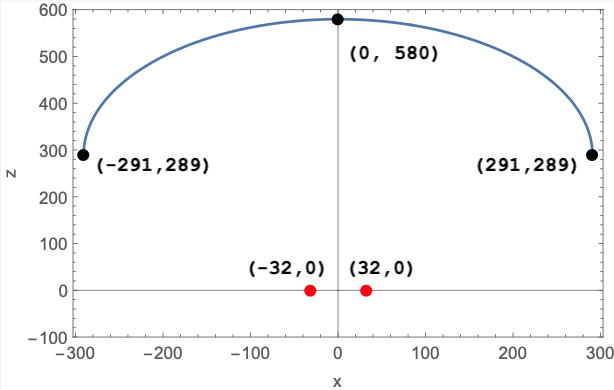
\includegraphics[width=0.6\textwidth]{figures/qib.png}
\end{figure}


\subsection*{(ii) Retinal Blur}
\subsubsection*{(a)}
The focal length can be calculated via:
\begin{equation}
    1/f = 1/D_e + 1/d_3,
\end{equation}
thus $f=\ 23.4$ mm. 
\subsubsection*{(b)}
For point $p_4$, the circle of confusion in the image plane can be calculated via the equation:
\begin{equation}
    c = S_e\frac{|d_4-d_3|}{|d_4|}\frac{f}{d_3-f} = 5f/(1000-f) = 0.12\ \text{mm}.
\end{equation}

\subsection*{(iii) Visual Acuity}
For 13.3'' Macbook Pro, the diagonal distance is 13.3''. With a screen resolution of $2560\times1600$, the diagonal has the number of pixel given as: $\sqrt{2560^2+1600^2}=3020$. Therefore the number of pixel in 1 cm is: $3020/33.78\ \text{cm} = 89.4\ \text{cm}^{-1}$. Therefore the visual angle of one pixel is $1/89.4/50/\pi\times180\degree = 0.0128\degree$. For 1 degree, at a viewing distance of 50 cm, the arc length will be $50\ cm \times \pi/180 = 0.873$ cm. The number of pixel that one can placed into such distance is: $0.873\times89.4 = 78$. Therefore the number of dark-bright alternating pair of lines is $78/2=39$ cpd. It is higher than 30 cpd that humans can perceive. 

\subsection*{(iv) Eccentricity and Visual Acuity}
\subsubsection*{(a,b)}
For p5, the angle $\theta_e=36.9\degree$. Using the equation of eccentricity, one can get: $\omega=m\theta_e+\omega_0 = 0.0275\times36.8+1/48 = 1.03\degree $. The acuity is the reciprocal of the MAR, therefore the highest frequency one can resolve would be: $1/1.03\degree=$ 0.97 cpd. 

\subsection*{2.4.4 Anaglyph Perceptual Question}
The alternative color scheme is such that the red color channel information from the left eye perspective is used for the red channel at the output, while the blue and green information from the right eye perspective is used for the blue and green channel at the output. The advantage is that it recovers certain amount of color information into the output image. However, the major disadvantage of such method is that false and unrealistic color will emerge at the edges where the color changes dramatically. In such region, the left and right images are shifted by a slight amount due to rendering. In between, the correct color for the two eyes should be different. However, using such method, it unifies the output color as a single one, which is incorrect for both eyes. 

\end{document}